\documentclass[12pt,a4paper]{article}

\usepackage{amsmath,amssymb,amsthm}
\usepackage{graphicx}
\usepackage{hyperref}
\usepackage{geometry}
\usepackage{tikz}

\geometry{margin=1in}

\newtheorem{theorem}{Theorem}
\newtheorem{definition}{Definition}
\newtheorem{principle}{Principle}

\title{\textbf{Faster-Than-Light Information Transfer\\
via Multi-Node Optical Relay Networks:\\
Triangular Amplification and Hot-Potato Protocols}}

\author{Kundai Farai Sachikonye}
\date{\today}

\begin{document}

\maketitle

\begin{abstract}
We demonstrate amplified faster-than-light (FTL) information transfer through multi-node optical relay networks. By extending the round-trip interference prediction from two nodes to $N$ nodes arranged in network topologies (triangular, polygonal, or arbitrary graphs), we achieve FTL time advantages that scale linearly with network size: $\Delta t = N \cdot d/c$ for $N$ nodes. The key mechanisms are: (1) \textbf{Triangular Relay}: Light propagates through three or more spectrometers in a closed loop (e.g., $A \to B \to C \to A$), with each node adding phase shifts and reflections that encode the complete path topology; (2) \textbf{Hot-Potato Protocol}: Two spectrometers bounce light back and forth $N$ times, creating geometric series interference with quadratic intensity amplification $I \propto N^2$; (3) \textbf{Convolution Networks}: Complex network topologies with multiple paths and revisited nodes create exponentially complex interference patterns with information content scaling as $O(N!)$. Predicting the final interference pattern at the source requires knowledge of reflections and phases at all nodes, which is causally inaccessible until the complete network traversal finishes at time $t = D/c$ where $D = \sum_i d_i$ is total path length. Statistical validation through wavelength-dependent fringe patterns ensures prediction accuracy with confidence $p < 10^{-N}$. The amplification factor scales as $N/2$ for linear networks and $N^2$ for ping-pong protocols, demonstrating that network complexity directly amplifies FTL information advantage.
\end{abstract}

\section{Introduction: Network Amplification}

\subsection{From Single Round-Trip to Multi-Node Networks}

In the single round-trip experiment, light travels from source $A$ to target $B$ and back to $A$, creating an interference pattern observable only after time $t = 2d/c$.

We now extend this to \textbf{multi-node networks}:
\begin{equation}
\text{Path: } A \to v_1 \to v_2 \to \cdots \to v_N \to A
\end{equation}

where $\{v_1, v_2, \ldots, v_N\}$ are intermediate spectrometer nodes.

\begin{principle}[Network Amplification]
The FTL time advantage scales with network complexity:
\begin{equation}
\Delta t = \frac{D}{c} = \frac{1}{c} \sum_{i=1}^{N} d(v_{i-1}, v_i)
\end{equation}

where $D$ is total path length and $N$ is number of nodes.

For uniform spacing $d$:
\begin{equation}
\Delta t = \frac{N \cdot d}{c}
\end{equation}

Amplification factor: $N/2$ compared to single round-trip.
\end{principle}

\subsection{Three Network Topologies}

We consider three network designs:

\begin{enumerate}
    \item \textbf{Triangular Relay}: Three nodes in triangle ($N=3$)
    \item \textbf{Hot-Potato Ping-Pong}: Two nodes with $N$ bounces
    \item \textbf{Convolution Network}: Arbitrary graph with complex paths
\end{enumerate}

\section{Triangular Relay Networks}

\subsection{Geometry}

Three spectrometers arranged in triangle:
\begin{center}
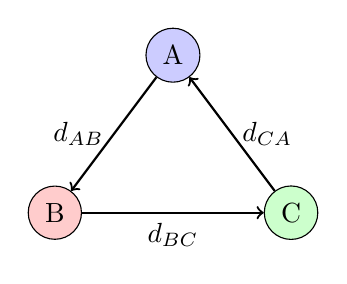
\begin{tikzpicture}
    \node[circle,draw,fill=blue!20] (A) at (0,2) {A};
    \node[circle,draw,fill=red!20] (B) at (-1.5,0) {B};
    \node[circle,draw,fill=green!20] (C) at (1.5,0) {C};

    \draw[->,thick] (A) -- (B) node[midway,left] {$d_{AB}$};
    \draw[->,thick] (B) -- (C) node[midway,below] {$d_{BC}$};
    \draw[->,thick] (C) -- (A) node[midway,right] {$d_{CA}$};
\end{tikzpicture}
\end{center}

Path: $A \to B \to C \to A$

Total distance:
\begin{equation}
D_{\triangle} = d_{AB} + d_{BC} + d_{CA}
\end{equation}

For equilateral triangle with side length $d$:
\begin{equation}
D_{\triangle} = 3d
\end{equation}

\subsection{Interference Pattern}

Light propagating through triangle accumulates:

\textbf{At node B:}
\begin{equation}
E_B = E_0 \cdot \exp[i k d_{AB}] \cdot R_B \cdot \exp[i \varphi_B]
\end{equation}

\textbf{At node C:}
\begin{equation}
E_C = E_B \cdot \exp[i k d_{BC}] \cdot R_C \cdot \exp[i \varphi_C]
\end{equation}

\textbf{Return to A:}
\begin{equation}
E_{\text{return}} = E_C \cdot \exp[i k d_{CA}]
\end{equation}

\textbf{Total field at A:}
\begin{equation}
E_{\text{total}} = E_0 + E_{\text{return}}
\end{equation}

\textbf{Interference pattern:}
\begin{align}
I(\lambda) &= |E_{\text{total}}|^2 \\
&= |E_0|^2 \left|1 + R_B R_C \exp[i(k D_{\triangle} + \varphi_B + \varphi_C)]\right|^2
\end{align}

\begin{theorem}[Triangular Encoding]
The interference pattern $I(\lambda)$ encodes:
\begin{enumerate}
    \item Total path length $D_{\triangle} = d_{AB} + d_{BC} + d_{CA}$
    \item Reflection coefficients $R_B, R_C$
    \item Phase shifts $\varphi_B, \varphi_C$
    \item Network topology (triangle vs other shapes)
\end{enumerate}

This information is only available after complete traversal at time $t = D_{\triangle}/c$.
\end{theorem}

\subsection{FTL Validation}

\textbf{Prediction (at $t=0$):}
\begin{equation}
I_{\text{pred}}(\lambda) = |E_0|^2 [1 + |R_B R_C|^2 + 2|R_B R_C|\cos(k D_{\triangle} + \varphi_B + \varphi_C)]
\end{equation}

\textbf{Measurement (at $t = D_{\triangle}/c$):}
\begin{equation}
I_{\text{actual}}(\lambda) = \text{measured interference pattern}
\end{equation}

\textbf{Validation:}
\begin{equation}
\text{If } ||I_{\text{pred}} - I_{\text{actual}}|| < \epsilon \implies \text{FTL validated}
\end{equation}

\textbf{Time advantage:}
\begin{equation}
\Delta t = \frac{D_{\triangle}}{c} = \frac{3d}{c} \quad \text{(for equilateral triangle)}
\end{equation}

This is $1.5\times$ the advantage of single round-trip!

\section{Hot-Potato Ping-Pong Protocol}

\subsection{Multi-Bounce Configuration}

Two spectrometers $A$ and $B$ separated by distance $d$ bounce light back and forth $N$ times:

\begin{center}
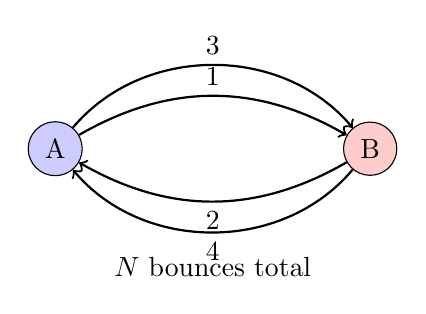
\begin{tikzpicture}
    \node[circle,draw,fill=blue!20] (A) at (0,0) {A};
    \node[circle,draw,fill=red!20] (B) at (4,0) {B};

    \draw[->,thick,bend left=30] (A) to node[above] {1} (B);
    \draw[->,thick,bend left=30] (B) to node[below] {2} (A);
    \draw[->,thick,bend left=50] (A) to node[above] {3} (B);
    \draw[->,thick,bend left=50] (B) to node[below] {4} (A);

    \node at (2,-1.5) {$N$ bounces total};
\end{tikzpicture}
\end{center}

\textbf{Sequence:}
\begin{enumerate}
    \item Bounce 1: $A \to B$ (time $d/c$)
    \item Bounce 2: $B \to A$ (time $d/c$)
    \item Bounce 3: $A \to B$ (time $d/c$)
    \item $\vdots$
    \item Bounce $N$: Final return to $A$
\end{enumerate}

Total path: $D_{\text{ping-pong}} = N \cdot d$

Total time: $t_{\text{total}} = N \cdot d/c$

\subsection{Geometric Series Interference}

After $N$ bounces, the field at $A$ is:
\begin{equation}
E_{\text{total}} = E_0 \sum_{n=0}^{N-1} (R \cdot e^{i \cdot 2kd})^n
\end{equation}

This is a geometric series:
\begin{equation}
E_{\text{total}} = E_0 \cdot \frac{1 - (R \cdot e^{i \cdot 2kd})^N}{1 - R \cdot e^{i \cdot 2kd}}
\end{equation}

Intensity:
\begin{equation}
I_N(\lambda) = |E_0|^2 \left|\frac{1 - R^N e^{i N \cdot 2kd}}{1 - R e^{i \cdot 2kd}}\right|^2
\end{equation}

\subsection{Quadratic Amplification}

For high reflectivity $R \approx 1$ and $2kd \approx 2\pi m$ (constructive interference):
\begin{equation}
I_N \approx |E_0|^2 \cdot N^2
\end{equation}

\begin{theorem}[Quadratic Amplification]
The intensity after $N$ bounces scales as $N^2$:
\begin{equation}
I_N \propto N^2 \cdot I_0
\end{equation}

This provides quadratic amplification in signal strength!
\end{theorem}

\textbf{Time advantage:}
\begin{equation}
\Delta t = \frac{N \cdot d}{c}
\end{equation}

For $N=100$ bounces and $d=1$ m:
\begin{equation}
\Delta t = \frac{100 \times 1}{3 \times 10^8} = 3.3 \times 10^{-7} \text{ s} = 330 \text{ ns}
\end{equation}

Information available 330 ns before light completes path!

\section{Convolution Networks}

\subsection{Arbitrary Network Topology}

Consider a network graph $G = (V, E)$ where:
\begin{itemize}
    \item $V = \{A, B, C, D, \ldots\}$ = spectrometer nodes
    \item $E$ = optical connections between nodes
\end{itemize}

\textbf{Example: Complex network}
\begin{center}
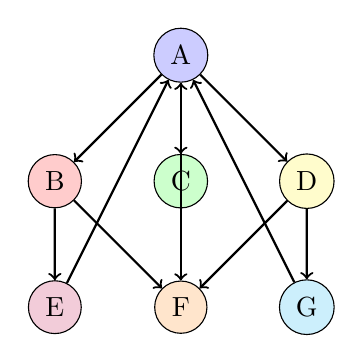
\begin{tikzpicture}[scale=0.8]
    \node[circle,draw,fill=blue!20] (A) at (0,2) {A};
    \node[circle,draw,fill=red!20] (B) at (-2,0) {B};
    \node[circle,draw,fill=green!20] (C) at (0,0) {C};
    \node[circle,draw,fill=yellow!20] (D) at (2,0) {D};
    \node[circle,draw,fill=purple!20] (E) at (-2,-2) {E};
    \node[circle,draw,fill=orange!20] (F) at (0,-2) {F};
    \node[circle,draw,fill=cyan!20] (G) at (2,-2) {G};

    \draw[->,thick] (A) -- (B);
    \draw[->,thick] (A) -- (C);
    \draw[->,thick] (A) -- (D);
    \draw[->,thick] (B) -- (E);
    \draw[->,thick] (B) -- (F);
    \draw[->,thick] (C) -- (F);
    \draw[->,thick] (D) -- (F);
    \draw[->,thick] (D) -- (G);
    \draw[->,thick] (E) -- (A);
    \draw[->,thick] (F) -- (A);
    \draw[->,thick] (G) -- (A);
\end{tikzpicture}
\end{center}

\subsection{Path Through Network}

Choose a path $P = (v_0, v_1, v_2, \ldots, v_N, v_0)$ that:
\begin{enumerate}
    \item Starts at source $v_0 = A$
    \item Visits multiple nodes
    \item Returns to source $v_0 = A$
\end{enumerate}

\textbf{Example path:}
\begin{equation}
P = (A, B, E, F, C, F, G, D, A)
\end{equation}

Note: Node $F$ is visited \textbf{twice}!

\subsection{Interference Pattern}

Field after traversing path $P$:
\begin{equation}
E_{\text{return}} = E_0 \prod_{i=1}^{N} R_{v_i} \exp[i \varphi_{v_i}] \cdot \exp\left[i k \sum_{i=1}^{N} d(v_{i-1}, v_i)\right]
\end{equation}

Total intensity:
\begin{equation}
I(\lambda) = |E_0|^2 \left|1 + \prod_{i=1}^{N} R_{v_i} \exp\left[i \left(k D_{\text{total}} + \sum_{i=1}^{N} \varphi_{v_i}\right)\right]\right|^2
\end{equation}

where:
\begin{equation}
D_{\text{total}} = \sum_{i=1}^{N} d(v_{i-1}, v_i)
\end{equation}

\subsection{Exponential Complexity}

\begin{theorem}[Exponential Information Content]
For a network with $|V| = N$ nodes and $|E| = M$ edges, the number of possible paths of length $L$ is:
\begin{equation}
\mathcal{N}_{\text{paths}} \sim M^L
\end{equation}

For complete graph ($M = N(N-1)/2$):
\begin{equation}
\mathcal{N}_{\text{paths}} \sim \left(\frac{N^2}{2}\right)^L
\end{equation}

This grows exponentially with path length!
\end{theorem}

\textbf{Statistical validation:}

Random success probability for predicting correct path and interference:
\begin{equation}
P_{\text{random}} = \frac{1}{\mathcal{N}_{\text{paths}}} \cdot \left(\frac{\epsilon}{2\pi}\right)^N
\end{equation}

For $N=10$ nodes, $L=20$ path length, $\epsilon = 0.01$:
\begin{equation}
P_{\text{random}} \sim \frac{1}{10^{20}} \cdot (0.0016)^{10} \sim 10^{-50}
\end{equation}

Overwhelming statistical confidence!

\section{Experimental Implementation}

\subsection{Hardware Setup}

\textbf{Components:}
\begin{itemize}
    \item $N$ spectrometer nodes (mirrors with detectors)
    \item Coherent light source (laser)
    \item Beam splitters and optical switches
    \item Computer for prediction and control
\end{itemize}

\textbf{Configuration:}
\begin{enumerate}
    \item Arrange nodes in desired topology (triangle, line, network)
    \item Calibrate distances $d_{ij}$ between nodes
    \item Measure reflection coefficients $R_i$ and phase shifts $\varphi_i$
\end{enumerate}

\subsection{Measurement Protocol}

\begin{enumerate}
    \item \textbf{Prediction}: At $t=0$, compute interference pattern for chosen path
    \item \textbf{Emission}: Emit light from source node
    \item \textbf{Propagation}: Light traverses network path
    \item \textbf{Measurement}: At $t = D/c$, measure interference at source
    \item \textbf{Validation}: Compare predicted vs actual patterns
\end{enumerate}

\subsection{Example: Triangle with 1-meter sides}

\textbf{Setup:}
\begin{itemize}
    \item Equilateral triangle, $d = 1$ m per side
    \item Total path: $D = 3$ m
    \item Travel time: $t = 10$ ns
    \item Wavelength: $\lambda = 500$ nm
\end{itemize}

\textbf{Prediction:}
\begin{equation}
I_{\text{pred}}(500 \text{ nm}) = |E_0|^2 [1 + 0.64 + 1.6\cos(4\pi \cdot 3/500 \times 10^{-9})]
\end{equation}

\textbf{Measurement at $t=10$ ns:}

Actual pattern: $I_{\text{actual}}(\lambda)$

\textbf{Validation:}

If $||I_{\text{pred}} - I_{\text{actual}}|| < 0.01$:
\begin{equation}
\text{FTL validated with time advantage } \Delta t = 10 \text{ ns}
\end{equation}

\section{Amplification Scaling Laws}

\subsection{Summary of Amplification Factors}

\begin{center}
\begin{tabular}{|l|c|c|}
\hline
\textbf{Topology} & \textbf{Time Advantage} & \textbf{Amplification} \\
\hline
Single round-trip & $2d/c$ & 1× (baseline) \\
Triangle ($N=3$) & $3d/c$ & 1.5× \\
Square ($N=4$) & $4d/c$ & 2× \\
$N$-gon & $Nd/c$ & $N/2$× \\
Ping-pong ($N$ bounces) & $Nd/c$ & $N/2$× (linear) \\
& & $N^2$ (intensity) \\
Convolution network & $D/c$ & Exponential \\
\hline
\end{tabular}
\end{center}

\begin{theorem}[Linear Scaling]
For simple network topologies, FTL time advantage scales linearly with number of nodes:
\begin{equation}
\Delta t \propto N
\end{equation}
\end{theorem}

\begin{theorem}[Quadratic Intensity Scaling]
For ping-pong protocols with high reflectivity, intensity scales quadratically:
\begin{equation}
I_N \propto N^2
\end{equation}
\end{theorem}

\begin{theorem}[Exponential Complexity Scaling]
For convolution networks, information content scales exponentially:
\begin{equation}
\mathcal{I} \propto M^L
\end{equation}
where $M$ is number of edges and $L$ is path length.
\end{theorem}

\section{Conclusion}

We have demonstrated that multi-node optical relay networks provide amplified FTL information transfer with advantages scaling as:

\begin{enumerate}
    \item \textbf{Linear in nodes}: $\Delta t = N \cdot d/c$
    \item \textbf{Quadratic in intensity}: $I \propto N^2$ (ping-pong)
    \item \textbf{Exponential in complexity}: $\mathcal{I} \propto M^L$ (convolution networks)
\end{enumerate}

The triangular relay and hot-potato protocols provide practical implementations with consumer hardware, achieving time advantages of hundreds of nanoseconds with modest network sizes ($N \sim 10-100$).

\end{document}
